\documentclass[11pt,a4paper,final,addpoints]{exam}
\usepackage[utf8]{inputenc}
\usepackage[portuguese]{babel}
\usepackage[T1]{fontenc}
\usepackage{amsmath}
\usepackage{amsfonts}
\usepackage{amssymb}
\usepackage{graphicx}
\usepackage{pstricks,pst-circ,pst-osci}
\usepackage[left=1cm,right=1cm,top=2cm,bottom=2cm,twoside]{geometry}
\author{Tiago Á. Oliveira}
\title{Relatorio Individual}


\pagestyle{headandfoot}

\extraheadheight[1.5in]{-.25in}

\firstpageheader{\textbf{Turma P9}}
%\firstpageheader{\textbf{Turma P13}}
{
\includegraphics[scale=1]{figs/logo_UA}
\linebreak\linebreak
\LARGE\textbf{Eletricidade \& Magnetismo}
\normalsize\linebreak
(2014-2015)
\linebreak\linebreak
\ifthenelse{\boolean{printanswers}}
{\textbf{Proposta de Resolu\c{c}\~{a}o do Relat\'{o}rio Individual de Laborat\'{o}rio}}
{\textbf{Relat\'{o}rio Individual de Laborat\'{o}rio}}
\linebreak
12 de dezembro de 2014
\linebreak}
{\textbf{Vers\~{a}o A}}
%{\textbf{Vers\~{a}o B}}

\runningheader{\oddeven{}{Eletricidade \& Magnetismo (2014-15)}}{}{\oddeven{Relat\'{o}rio Individual de Laborat\'{o}rio}{}}
\headrule

\footrule
\firstpagefooter{\emph{Revis\~{a}o: \today}}{}{P\'{a}gina \thepage}
\runningfooter{\oddeven{}{P\'{a}gina \thepage}}{\iflastpage{Fim!}}{\oddeven{P\'{a}gina \thepage}}

% RESPOSTAS 
\printanswers
\renewcommand{\solutiontitle}{\noindent\textbf{Resposta:\newline}}


\begin{document}
\boxedpoints
\pointsinmargin

\ifprintanswers
\noindent\textbf{Cota\c{c}\~{o}es:}
\begin{center}
\hqword{\textit{Quest\~{a}o}}
\hpword{\textit{Pontos}}
\hsword{\textit{Obtidos}}
\htword{\textbf{Total}}
\gradetable[h][questions]
\linebreak
\end{center}
\else
\begin{center}
\makebox[\textwidth]{\textbf{Nome:}~\underline{\hspace{11cm}}~\textbf{N.\textsuperscript{o} Mecanogr\'{a}fico:}~\underline{\hspace{2.5cm}}}
\end{center}

\noindent\textbf{Recomenda\c{c}\~{o}es:}
\begin{itemize}
\item O relat\'{o}rio \'{e} realizado individualmente;

\item Leia atentamente todo o enunciado da prova e se tiver d\'{u}vidas coloque-as ao docente;

\item Tem a dura\c{c}\~{a}o exata de 2 horas, sem qualquer toler\^{a}ncia;

\item O enunciado do relat\'{o}rio tem 2 vers\~{o}es distintas mas de igual dificuldade. 

\underline{Dever\~{a}o indicar a vers\~{a}o (A ou B) no in\'{i}cio da folha de resposta};

\item \underline{Dever\~{a}o justificar todas as respostas};

\item N\~{a}o ser\'{a} permitida a consulta dos guias, fichas ou dos registos efetuados durante as aulas;

\item N\~{a}o haver\'{a} formul\'{a}rio para as leis fundamentais (Lei de Ohm, Kirschoff, Faraday, Lenz, etc.). Equa\c{c}\~{o}es de dedu\c{c}\~{a}o complexa/demorada, caso sejam necess\'{a}rias, estar\~{a}o presentes no enunciado;

\item Podem usar m\' {a}quina de calcular com capacidades gr\'{a}ficas;

\item O uso do computador/tablet est\'{a} restringido apenas para uso no tratamento de dados (Excel, MatLAB, etc.) n\~{a}o podendo ser usado para consulta de PDF's ou liga\c{c}\~{a}o \`{a} Internet;

\item O telem\'{o}vel dever\'{a} estar desligado durante a prova.
\end{itemize}

\noindent\textbf{Cota\c{c}\~{o}es:}
\begin{center}
\hqword{\textit{Quest\~{a}o}}
\hpword{\textit{Pontos}}
\hsword{\textit{Obtidos}}
\htword{\textbf{Total}}
\gradetable[h][questions]
\linebreak
\end{center}

\noindent\textbf{Constantes fundamentais:}
\begin{center}
\begin{tabular}{cc}
$\varepsilon_0 = 8.85\times10^{-12}~\text{C}^2/\text{Nm}^2$ & $\mu_0 = 4\pi\times10^{-7}~\text{N}/\text{A}^2$ \\ 
$e=1.60\times10^{-19}~\text{C}$ & $m_e=9.11\times10^{-31}~\text{kg}$ \\ 
\end{tabular} 
\end{center}

\newpage
\fi

\begin{questions}
% Versao P9 - A
%
%

\question
\textbf{Trabalho Pr\'{a}tico 4 : Circuito RC}

Recorde o Trabalho Pr\'{a}tico 4, no qual estudou a resposta transit\'{o}ria do circuito RC.

Neste trabalho procedeu ao carregamento de um condensador, com capacidade conhecida $C=10~000\pm 20\%~\mu\text{F}$, usando o circuito da Fig.~\ref{fig:cargcond} e registou na Tabela~\ref{tab:vcondensador} a d.d.p. nos terminais do condensador em fun\c{c}\~{a}o do tempo $v_C\left(t\right)$.

\begin{figure}[h]
\centering
\begin{pspicture}[showgrid=false](11,5)
\pnodes(1,1){A}(1,4){B}(3,4){C}(6,4){D}(6,1){E}(9,4){F}(9,1){G}
\vdc[labeloffset=1.1](B)(A){$15~\text{V}$}
\newSwitch[ison=true](B)(C){$S_1$}
\newSwitch[ison=true](D)(F){$S_2$}
\resistor[dipolestyle=zigzag](C)(D){$R_1=1k5$}
\resistor[dipolestyle=zigzag,labeloffset=-1.3](D)(E){$R_2=1k$}
\capacitor[dipolestyle=chemical,
           labeloffset=-1,
           tension,
           tensionlabel=$v_C\left(t\right)$,
           tensionlabeloffset=1.5](F)(G){$C$}
\wire(A)(E)
\wire(E)(G)
\newground(E)
\end{pspicture}
\caption{\label{fig:cargcond}Circuito de carregamento do condensador.}
\end{figure}

\begin{table}[h]
\centering
\caption{\label{tab:vcondensador}Tens\~{a}o ($v_C$) nos terminais do condensador em fun\c{c}\~{a}o do instante de tempo ($t$).}
\begin{tabular}{|c|c|c|c|c|c|c|}
\hline 
$t\pm 1$ (s) & 0 & 6 & 12 & 18 & 24 & 30 \\ 
\hline 
$v_C\pm 0.01$ (V) & 0.02 & 3.80 & 5.18 & 5.70 & 5.88 & 5.96 \\ 
\hline 
\end{tabular} 
\end{table}

\begin{parts}
\part[25]
Sabendo que a d.d.p. nos terminais do condensador cresce exponencialmente, segundo a Eq.~\ref{eq:vcarga}, linearize esta express\~{a}o e determine experimentalmente a constante de tempo de carga do condensador $\tau$ e respetivo erro associado $\Delta\tau$, usando as medidas experimentais diretas presentes na Tabela~\ref{tab:vcondensador}.

Nota: N\~{a}o precisa de representar graficamente os pontos experimentais e a reta da lineariza\c{c}\~{a}o.


\begin{equation}
\label{eq:vcarga}
v_C\left(t\right)=\varepsilon\left[1-e^{\left(-\frac{t}{\tau}\right)}\right]
\end{equation}
\begin{solution}
\emph{Proposta de lineariza\c{c}\~{a}o da Eq.~\ref{eq:vcarga}:}
\begin{equation*}
v_C\left(t\right)=\varepsilon\left[1-e^{\left(-\frac{t}{\tau}\right)}\right]
\Leftrightarrow
\frac{v_C\left(t\right)}{\varepsilon}=\left[1-e^{\left(-\frac{t}{\tau}\right)}\right]
\Leftrightarrow
\frac{v_C\left(t\right)}{\varepsilon}-1=-e^{\left(-\frac{t}{\tau}\right)}
\Leftrightarrow
1-\frac{v_C\left(t\right)}{\varepsilon}=e^{\left(-\frac{t}{\tau}\right)}
\Leftrightarrow
\end{equation*}
\begin{equation*}
\ln{\left[1-\frac{v_C\left(t\right)}{\varepsilon}\right]}=-\frac{t}{\tau}
\Leftrightarrow
-t=\tau\ln{\left[1-\frac{v_C\left(t\right)}{\varepsilon}\right]}
\end{equation*}
\begin{equation*}
y=-t~,~x=\ln{\left[1-\frac{v_C\left(t\right)}{\varepsilon}\right]}~,~m=\tau~,~b=0
\end{equation*}

Deve-se sempre confirmar que $\Delta y \gg |m \Delta x|$, mas por falta de outros conhecimentos, avan\c{c}a-se com a analise.

\emph{M\'{e}todo dos M\'{i}nimos Desvios Quadrados (MMDQ):}
\begin{equation*}
m=\tau~,~b=0~,r^2=
\end{equation*}
\end{solution}

\part[15]
Explique qual o significado f\'{i}sico da constante de tempo de carregamento do condensador $\tau$. Pode recorrer a esbo\c{c}os gr\'{a}ficos, caso lhe seja conveniente.

\begin{solution}
\begin{center}
\begin{pspicture}[showgrid=false](-1.5,-0.5)(9,3.5)
\psset{xunit=0.3cm,yunit=0.3cm}
\psplot[plotpoints=10,linecolor=blue]{0}{6}{10 x mul 6 div}
\psline[linecolor=blue,linestyle=dashed,dash=3pt 2pt](6,10)(6,0)
\psplot[linecolor=red,plotpoints=100]{0}{30}{10 1 Euler x 6 div neg exp sub mul}
\psline{->}(0,0)(0,12)
\psline{->}(0,0)(30,0)
\psline[linestyle=dashed,dash=3pt 2pt](0,10)(30,10)
\psline[linecolor=red,linestyle=dashed,dash=3pt 2pt](0,6.3)(6,6.3)
\rput[tl](30,0){$t$}
\rput[br](0,12){$v_C$}
\rput[t](6,-0.5){$\tau$}
\rput[r](-0.5,10){$\varepsilon$}
\rput[r](-0.5,6.3){$\left[1-\frac{1}{e}\right]\varepsilon$}
\rput[r](-0.5,4.6){$\sim 63\%~\varepsilon$}
\end{pspicture}
\end{center}
Na hipotese de que o carregamento do condensador tenha um comportamento linear (curva a \textcolor{blue}{azul}), a contante de tempo $\tau$ ser\'{a} o tempo necess\'{a}rio a este ficar totalmente carregado. Contudo, como o condensador exibe um comportamento exponencial de carregamento (curva a \textcolor{red}{vermelho}), a contante de tempo $\tau$ corresponde ao tempo necess\'{a}rio ao condensador a adquirir $\left[1-\frac{1}{e}\right]$ (ou seja, $\sim 63\%$) da carga m\'{a}xima.
\end{solution}

\part[10]
De que modo teria de alterar o circuito da Fig.~\ref{fig:cargcond} para aumentar o valor da constante de tempo de carregamento do condensador $\tau$?

\begin{solution}
Atendendo ao circuito da Fig.~\ref{eq:vcarga}, a constante de tempo de carregamento do condensador \'{e} dada por $\tau=(R_1||R_2)C$. Para aumentar esta grandeza, mantendo a capacidade do condensador, teria que se alterar as resist\^{e}ncias, no seu conjunto ou isoladamente, de modo que a associa\c{c}\~{a}o de resist\^{e}ncias $R_1||R_2$ aumentasse o seu valor.
\end{solution}
\end{parts}
\question
\textbf{Trabalho Pr\'{a}tico 6 : Indu\c{c}\~{a}o Eletromagn\'{e}tica}

Recorde o trabalho pr\'{a}tico sobre a Indu\c{c}\~{a}o eletromagn\'{e}tica.

\begin{parts}
\part[10]
Na primeira parte deste trabalho montou o circuito da Fig.~\ref{fig:bobinas}, com o objetivo de estudar a Lei de Faraday e de Lenz, na qual se varia o fluxo magn\'{e}tico atrav\'{e}s de uma bobina quando esta est\'{a} em movimento relativo a uma outra, percorrida por uma corrente $I$.

Descreva o que observou no movimento dos ponteiros do galvan\'{o}metro, quando afastou a bobina 2 e, \`{a} luz das leis de Faraday e de Lenz, indique o sentido da corrente induzida no circuito da bobina 2.

\begin{figure}[h]
\centering
\begin{pspicture}[showgrid=false](9,5)
\pnodes(1,1){A}(1,4){B}(4,4){C}(4,1){D}(5,1){E}(5,4){F}(8,4){G}(8,1){H}
\vdc[labeloffset=1](A)(D){$15~\text{V}$}
\resistor[dipolestyle=zigzag,labelangle=:U](A)(B){$5~\Omega$}
\coil[dipolestyle=curved,
      intensitylabel=$I$,
      tensionlabel=Bobina 1,
      tensioncolor=white,
      tensionlabeloffset=0.7,
      labeloffset=-.5](B)(C){$1200~\text{esp.}$}
\wire(C)(D)

\wire(E)(F)
\coil[dipolestyle=curved,
      tensionlabel=Bobina 2,
      tensionlabeloffset=0.7,
      labeloffset=-.5](F)(G){$3600~\text{esp.}$}
\wire(G)(H)
\circledipole[labeloffset=0](E)(H){\Large\textbf{G}}

\end{pspicture}
\caption{\label{fig:bobinas}}
\end{figure}

\begin{solution}

\end{solution}

\part\label{part:m}
Considere um circuito no qual est\~{a}o ligados em s\'{e}rie um gerador de sinal, uma resist\^{e}ncia de $R=100~\Omega$ e um solenoide de raio $r=1.38~\text{cm}$ e $N/l=3000$ espiras por metro. Uma bobina de $N_b=1200$ espiras envolve o solenoide.
\begin{subparts}
\subpart[20]
Sabendo que a for\c{c}a eletromotriz (f.e.m.) induzida na bobina dada pela Eq.~\ref{eq:fem}, determine o coeficiente de indu\c{c}\~{a}o m\'{u}tua esperado.

\begin{equation}
\label{eq:fem}
\varepsilon=\pi\mu_0\frac{N}{l}r^2N_b\frac{\mathrm d i}{\mathrm d t}
\end{equation}

\begin{solution}
Como $\varepsilon=M\frac{\mathrm d i}{\mathrm d t}$, facilmente se infere da Eq.~\ref{eq:fem} que o coeficiente de indu\c{c}\~{a}o m\'{u}tua esperado \'{e} dado por:
\begin{equation*}
M=\pi\mu_0\frac{N}{l}r^2N_b
\end{equation*}
\end{solution}
\end{subparts}

\part 
Considere um circuito no qual est\~{a}o ligados em s\'{e}rie um gerador de sinal e uma bobina ($1200~\text{espiras}$, resist\^{e}ncia de $13~\Omega$ e coeficiente de auto-indut\^{a}ncia $L=54~\text{mH}$.)

Aplicou-se um sinal sinusoidal \`{a} bobina, observando-o no Canal A do oscilosc\'{o}pio (Fig~\ref{fig:osci}. - \textit{tracejado}) tendo-se observado no Canal B dos oscilosc\'{o}pio (Fig~\ref{fig:osci}. - \textit{cheio}) o sinal induzido no solenoide.

\begin{figure}[h]
\begin{center}
\newpsstyle{Dash}{linestyle=dashed,
linecolor=black,linewidth=0.035,plotpoints=50}
\psscalebox{1}{
\Oscillo[Wave1=\SinusA,
         Wave2=\SinusB,
    amplitude1=15.5,
    amplitude2=1.2,
       period1=.44,
       period2=.44,
        phase1=0.0,
        phase2=0.0,        
    sensivity1=5.0,
    sensivity2=1.0,
       timediv=0.1,       
    plotstyle1=Dash,
      AllColor=false]}
\caption{\label{fig:osci}Visor do oscilosc\'{o}pio. O Canal A est\'{a} representado a tracejado enquanto o Canal B a cheio.}
\end{center}
\end{figure}

\begin{subparts}
\subpart[25]
Calcule o coeficiente de indu\c{c}\~{a}o m\'{u}tua do circuito e compare-o com o valor obtido em~(\ref{part:m}). 
\begin{solution}

\end{solution}

\subpart[20]
Se o sinal aplicado (Canal A) fosse quadrangular, o sinal induzido (Canal B) seria triangular? \underline{Justifique} a sua resposta.
\begin{solution}
N\~{a}o. Como j\'{a} se constatou em al\'{i}neas anteriores, a f.e.m. induzida $\varepsilon\propto\frac{\mathrm d i}{\mathrm d t}$ logo se o sinal aplicado \'{e} de forma quadrangular, a sua derivada \'{e} nula nos patamares extremos dos sinais, havendo apenas descuntinuidade na transi\c{c}\~{a}o da componente positiva para a negativa (e vice-versa) do sinal aplicado. Isso traduzirar-se ia num sinal induzido praticamente nulo, apresentando descontinuidades.
\end{solution}
\end{subparts}
\end{parts}
\newpage
\question
\textbf{Trabalho Pr\'{a}tico 5 : Bobinas de Helmholtz}

Recorde o trabalho pr\'{a}tico sobre o estudo do campo magn\'{e}tico produzido pelas Bobinas de Helmholtz. Os resultados experimentais obtidos est\~{a}o representados no gr\'{a}fico da Fig.~\ref{fig:helmholtz}. Cada bobina tem de raio $R=3.5~\text{cm}$.

\begin{figure}[ht]
\centering
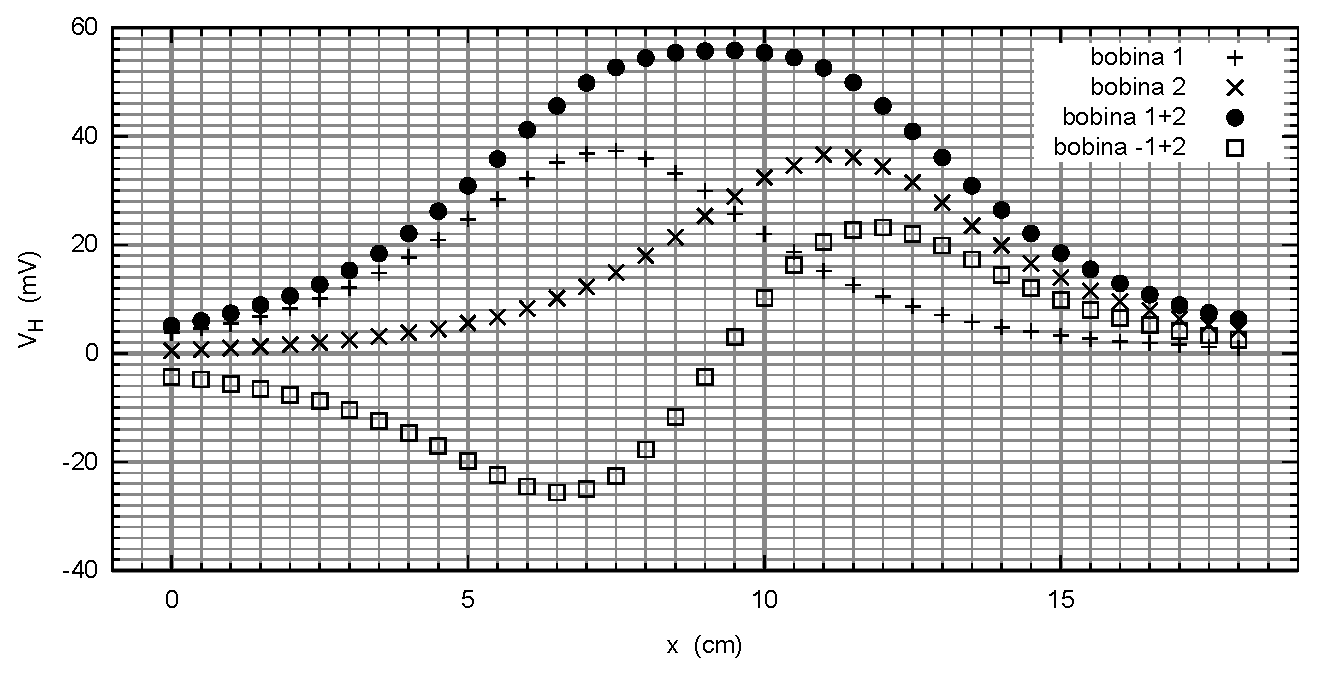
\includegraphics[scale=0.8]{gnuplot/helmholtz.eps}
\caption{\label{fig:helmholtz}Tens\~{a}o de Hall ao longo do eixo das bobinas.}
\end{figure}

\begin{parts}
\part[20]
A medi\c{c}\~{a}o do campo foi feita com recurso a uma sonda de efeito de Hall. Justifique a necessidade de proceder \`{a} sua calibra\c{c}\~{a}o e explique como fez essa calibra\c{c}\~{a}o.

\begin{solution}

\end{solution}

\part[15]
Sabendo que a constante de calibra\c{c}\~{a}o da sonda $C_c \pm \Delta Cc = 34.9 \pm 0.5~\text{(mT/V)}$, determine o valor do campo magn\'{e}tico para a Bobina 2 e respetivo erro, na posi\c{c}\~{a}o $x=11.5~\text{cm}$.

\begin{solution}

\end{solution}

\part[10]
Indique, justificando, se trabalhou em configura\c{c}\~{a}o de Helmholtz e indique tamb\'{e}m uma possivel aplica\c{c}\~{a}o para esta configura\c{c}\~{a}o de bobinas.

\begin{solution}

\end{solution}

\part[15]
Conclua, atrav\'{e}s do gr\'{a}fico, se se verifica ou n\~{a}o o princ\'{i}pio da sobreposi\c{c}\~{a}o do campo magnetico no caso em que as bobinas t\^{e}m corrente a fluir em sentidos opostos.

\begin{solution}

\end{solution}

\part[15]
Determine a corrente aplicada na bobina 2 se esta tiver $200~\text{espiras}$, sabendo que o campo magn\'{e}tico por uma espira ao longo do seu eixo \'{e} dado pela Eq.~\ref{eq:coilfield}.

\begin{equation}
\label{eq:coilfield}
B\left(x\right)=\frac{\mu_0}{2}\frac{IR^2}{\left(R^2+x^2\right)^{3/2}}
\end{equation}

\begin{solution}

\end{solution}
\end{parts}

% Versao P9 - B
%%
%

\question
\textbf{Trabalho Pr\'{a}tico 4 : Circuito RC}

Recorde o Trabalho Pr\'{a}tico 4, no qual estudou a resposta transit\'{o}ria do circuito RC.

Neste trabalho procedeu ao descarregamento de um condensador, com capacidade conhecida $C=10~000\pm 20\%~\mu\text{F}$, usando o circuito da Fig.~\ref{fig:descargcond} e registou na Tabela~\ref{tab:vcondensador} a d.d.p. nos terminais do condensador em fun\c{c}\~{a}o do tempo $v_D\left(t\right)$.

\begin{figure}[h]
\centering
\begin{pspicture}[showgrid=false](11,5)
\pnodes(1,1){A}(1,4){B}(3,4){C}(6,4){D}(6,1){E}(9,4){F}(9,1){G}
\vdc[labeloffset=1.1](B)(A){$15~\text{V}$}
\newSwitch[ison=false](B)(C){$S_1$}
\newSwitch[ison=true](D)(F){$S_2$}
\resistor[dipolestyle=zigzag](C)(D){$R_1=1k5$}
\resistor[dipolestyle=zigzag,labeloffset=-1.3](D)(E){$R_2=1k$}
\capacitor[dipolestyle=chemical,
           labeloffset=-1,
           tension,
           tensionlabel=$v_D\left(t\right)$,
           tensionlabeloffset=1.5](F)(G){$C$}
\wire(A)(E)
\wire(E)(G)
\newground(E)
\end{pspicture}
\caption{\label{fig:descargcond}Circuito de descarregamento do condensador.}
\end{figure}

\begin{table}[h]
\centering
\caption{\label{tab:vcondensador}Tens\~{a}o ($v_D$) nos terminais do condensador em fun\c{c}\~{a}o do instante de tempo ($t$).}
\begin{tabular}{|c|c|c|c|c|c|c|c|c|c|c|}
\hline 
$t\pm 1$ (s) & 0 & 6 & 12 & 18 & 24 & 30 & 36 & 42 & 48 & 54\\ 
\hline 
$v_D\pm 0.01$ (V) & 5.95 & 3.29 & 1.81 & 0.99 & 0.54 & 0.29 & 0.16 & 0.09 & 0.04 & 0.03\\ 
\hline 
\end{tabular} 
\end{table}

\begin{parts}
\part[25]
Sabendo que a d.d.p. nos terminais do condensador decresce exponencialmente, segundo a Eq.~\ref{eq:vdescarga}, linearize esta express\~{a}o e determine experimentalmente a constante de tempo de descarga do condensador $\tau$ e respetivo erro associado $\Delta\tau$, usando as medidas experimentais diretas presentes na Tabela~\ref{tab:vcondensador}.

Nota: N\~{a}o precisa de representar graficamente os pontos experimentais e a reta da lineariza\c{c}\~{a}o.

\begin{equation}
\label{eq:vdescarga}
v_D\left(t\right)=\varepsilon\left[e^{\left(-\frac{t}{\tau}\right)}\right]
\end{equation}

\part[15]
Explique qual o significado f\'{i}sico da constante de tempo de descarregamento do condensador $\tau$. Pode recorrer a esbo\c{c}os gr\'{a}ficos, caso lhe seja conveniente.

\begin{solution}

\begin{pspicture}[showgrid=false](-1.5,-0.5)(9,3.5)
\psset{xunit=0.3cm,yunit=0.3cm}
\psplot[plotpoints=10,linecolor=blue]{0}{6}{10 10 x mul 6 div sub}
\psline[linecolor=blue,linestyle=dashed,dash=3pt 2pt](6,3.7)(6,0)
\psplot[linecolor=red,plotpoints=100]{0}{30}{10 Euler x 6 div neg exp mul}
\psline{->}(0,0)(0,12)
\psline{->}(0,0)(30,0)
\psline[linecolor=red,linestyle=dashed,dash=3pt 2pt](0,3.7)(6,3.7)
\rput[tl](30,0){$t$}
\rput[br](0,12){$v_D$}
\rput[t](6,-0.5){$\tau$}
\rput[r](-0.5,10){$\varepsilon$}
\rput[r](-0.5,3.7){$\frac{\varepsilon}{e}$}
\rput[r](-0.5,2.2){$\approx37\%~\varepsilon$}
\end{pspicture}

\end{solution}

\part[10]
De que modo teria de alterar o circuito da Fig.~\ref{fig:descargcond} para aumentar o valor da tens\~{a}o inicial do condensador $v_D(t=0)$?
\end{parts}
%\question
\textbf{Trabalho Pr\'{a}tico 6 : Indu\c{c}\~{a}o Eletromagn\'{e}tica}

Recorde o trabalho pr\'{a}tico sobre a Indu\c{c}\~{a}o eletromagn\'{e}tica.

\begin{parts}
\part[10]
Na primeira parte deste trabalho montou o circuito da Fig.~\ref{fig:bobinas}, com o objetivo de estudar a Lei de Faraday e de Lenz, na qual se varia o fluxo magn\'{e}tico atrav\'{e}s de uma bobina usando um \'{i}man.

\begin{subparts}
\subpart
Descreva o que observou no movimento dos ponteiros do galvan\'{o}metro, quando aproximou o \'{i}man \`{a} bobina e, \`{a} luz das leis de Faraday e de Lenz, indique o sentido da corrente induzida no circuito da bobina.

\subpart E quando afastou o \'{i}man da bobina?
\end{subparts}

\begin{figure}[h]
\centering
\begin{pspicture}[showgrid=false](8,4)
\pnodes(1,1){A}(1,3){B}(7,3){C}(7,1){D}

\wire(A)(B)
\coil[dipolestyle=curved,
      labeloffset=-.5](B)(C){$1200~\text{esp.}$}
\pspolygon[fillcolor=red,fillstyle=solid](1.2,2.8)(2,2.8)(2,3.2)(1.2,3.2)
\rput*[t]{0}(1.6,2.6){S}
\pspolygon[fillcolor=blue,fillstyle=solid](2,2.8)(2.8,2.8)(2.8,3.2)(2,3.2)
\rput*[t]{0}(2.4,2.6){N}
\psline[linewidth=2pt]{<->}(1.5,3.5)(2.5,3.5)
\wire(C)(D)
\circledipole[labeloffset=0](A)(D){\Large\textbf{G}}

\end{pspicture}
\caption{\label{fig:bobinas}}
\end{figure}

\part\label{part:m}
Considere um circuito no qual est\~{a}o ligados em s\'{e}rie um gerador de sinal, uma resist\^{e}ncia de $R=100~\Omega$ e um solenoide de raio $r=1.38~\text{cm}$ e $N/l=3000$ espiras por metro. Uma bobina de $N_b=1200$ espiras envolve o solenoide.
\begin{subparts}
\subpart[20]
Sabendo que a for\c{c}a eletromotriz (f.e.m.) induzida na bobina dada pela Eq.~\ref{eq:fem}, determine o coeficiente de indu\c{c}\~{a}o m\'{u}tua esperado.

\begin{equation}
\label{eq:fem}
\varepsilon=\pi\mu_0\frac{N}{l}r^2N_b\frac{\mathrm d i}{\mathrm d t}
\end{equation}

\end{subparts}

\part 
Considere um circuito no qual est\~{a}o ligados em s\'{e}rie um gerador de sinal e uma bobina ($1200~\text{espiras}$, resist\^{e}ncia de $13~\Omega$ e coeficiente de auto-indut\^{a}ncia $L=54~\text{mH}$.)

Aplicou-se um sinal sinusoidal \`{a} bobina, observando-o no Canal A do oscilosc\'{o}pio (Fig~\ref{fig:osci}. - \textit{tracejado}) tendo-se observado no Canal B dos oscilosc\'{o}pio (Fig~\ref{fig:osci}. - \textit{cheio}) o sinal induzido no solenoide.

\begin{figure}[h]
\begin{center}
\newpsstyle{Dash}{linestyle=dashed,
linecolor=black,linewidth=0.035,plotpoints=50}
\psscalebox{1}{
\Oscillo[Wave1=\SinusA,
         Wave2=\SinusB,
    amplitude1=15.5,
    amplitude2=1.2,
       period1=.44,
       period2=.44,
        phase1=0.0,
        phase2=0.0,        
    sensivity1=5.0,
    sensivity2=1.0,
       timediv=0.1,       
    plotstyle1=Dash,
      AllColor=false]}
\caption{\label{fig:osci}Visor do oscilosc\'{o}pio. O Canal A est\'{a} representado a tracejado enquanto o Canal B a cheio.}
\end{center}
\end{figure}

\begin{subparts}
\subpart[25]
Calcule o coeficiente de indu\c{c}\~{a}o m\'{u}tua do circuito e compare-o com o valor obtido em~(\ref{part:m}), 

\subpart[20]
Se o sinal induzido (Canal B) fosse praticamente constante no tempo, o sinal aplicado (Canal A) seria triangular? \underline{Justifique} a sua resposta.

\end{subparts}
\end{parts}
%\newpage
%\question
\textbf{Trabalho Pr\'{a}tico 5 : Bobinas de Helmholtz}

Recorde o trabalho pr\'{a}tico sobre o estudo do campo magn\'{e}tico produzido pelas Bobinas de Helmholtz. Os resultados experimentais obtidos est\~{a}o representados no gr\'{a}fico da Fig.~\ref{fig:helmholtz}. Cada bobina tem de raio $R=3.5~\text{cm}$.

\begin{figure}[ht]
\centering
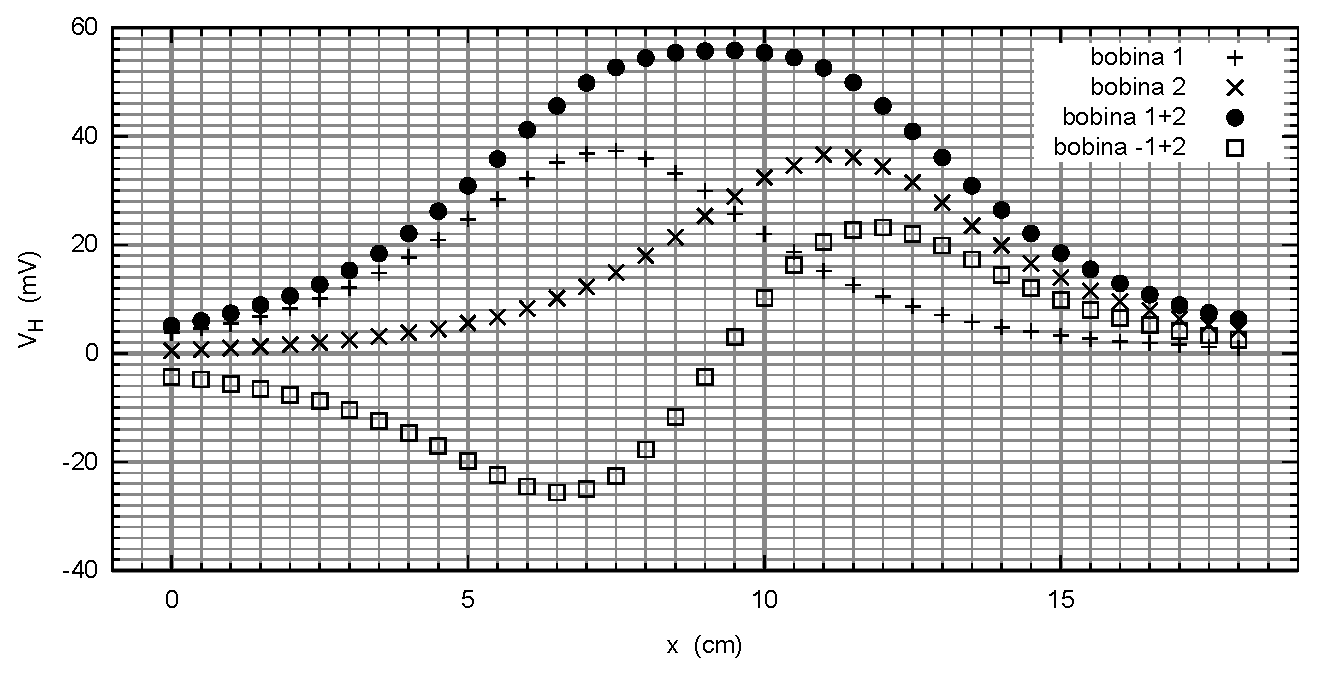
\includegraphics[scale=0.8]{gnuplot/helmholtz.eps}
\caption{\label{fig:helmholtz}Tens\~{a}o de Hall ao longo do eixo das bobinas.}
\end{figure}

\begin{parts}
\part[20]
A medi\c{c}\~{a}o do campo foi feita com recurso a uma sonda de efeito de Hall. Explique o que \'{e} o efeito de Hall num semicondutor cujos portadores de carga maiorit\'{a}rios s\~{a}o negativos. (Nota: Pode recorrer a esbo\c{c}o gr\'{a}fico para ilustrar a sua resposta.)

\part[15]
Sabendo que a constante de calibra\c{c}\~{a}o da sonda $C_c \pm \Delta Cc = 34.9 \pm 0.5~\text{(mT/V)}$, determine o valor do campo magn\'{e}tico para a Bobina 1 e respetivo erro, na posi\c{c}\~{a}o $x=7.5~\text{cm}$.

\part[10]
Indique, justificando, se trabalhou em configura\c{c}\~{a}o de Helmholtz e indique tamb\'{e}m uma possivel aplica\c{c}\~{a}o para esta configura\c{c}\~{a}o de bobinas.

\part[15]
Conclua, atrav\'{e}s do gr\'{a}fico, se se verifica ou n\~{a}o o princ\'{i}pio da sobreposi\c{c}\~{a}o do campo magnetico no caso em que as bobinas t\^{e}m corrente a fluir no mesmo sentido.

\part[15]
Determine a corrente aplicada na bobina 1 se esta tiver $200~\text{espiras}$, sabendo que o campo magn\'{e}tico por uma espira ao longo do seu eixo \'{e} dado pela Eq.~\ref{eq:coilfield}.

\begin{equation}
\label{eq:coilfield}
B\left(x\right)=\frac{\mu_0}{2}\frac{IR^2}{\left(R^2+x^2\right)^{3/2}}
\end{equation}
\end{parts}

\end{questions}
\end{document}